\section{Theory}
\label{section: Chapter4/theory}

paragraph reviewing physical system

In Chapter \ref{Chapter3}, the mathematical model for single-phase fluid-driven fracture is described in Section \ref{formulation}. In what follows, this same model is assumed, as all derivations are independent of the system dimensionality as well as fracture shapes. More precisely, since the multi-resolution framework will be used, two coexisting descriptions are used. In a global domain, cracks are assumed to be represented by two-dimensional surfaces embedded in the 3D domain and the governing equations and boundary condition are those from \eqref{linear momentum balance} - \eqref{pf_ic}. In the local domain, which will be described next, the fracture problem is treated with a variational phase-field formulation, given by \eqref{basic u problem}-\eqref{eq:ddot-strong}.

MR overview

crack propagation treatment, describing useful entities and quantities

algorithm summary and figures

some results

\begin{figure}[h]
    \centering
    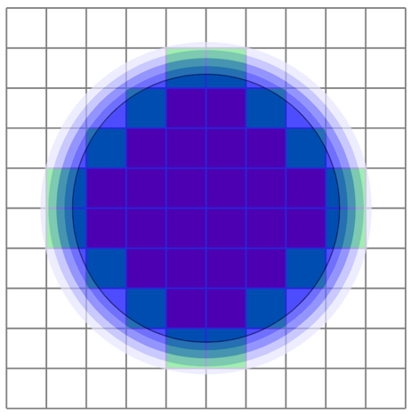
\includegraphics[width=0.5\linewidth]{Chapter4/figures/blue_circle.png}
    \caption{Multi-resolution solution algorithm.}
    \label{fig:lorem1}
\end{figure}


\begin{figure}[h]
    \centering
    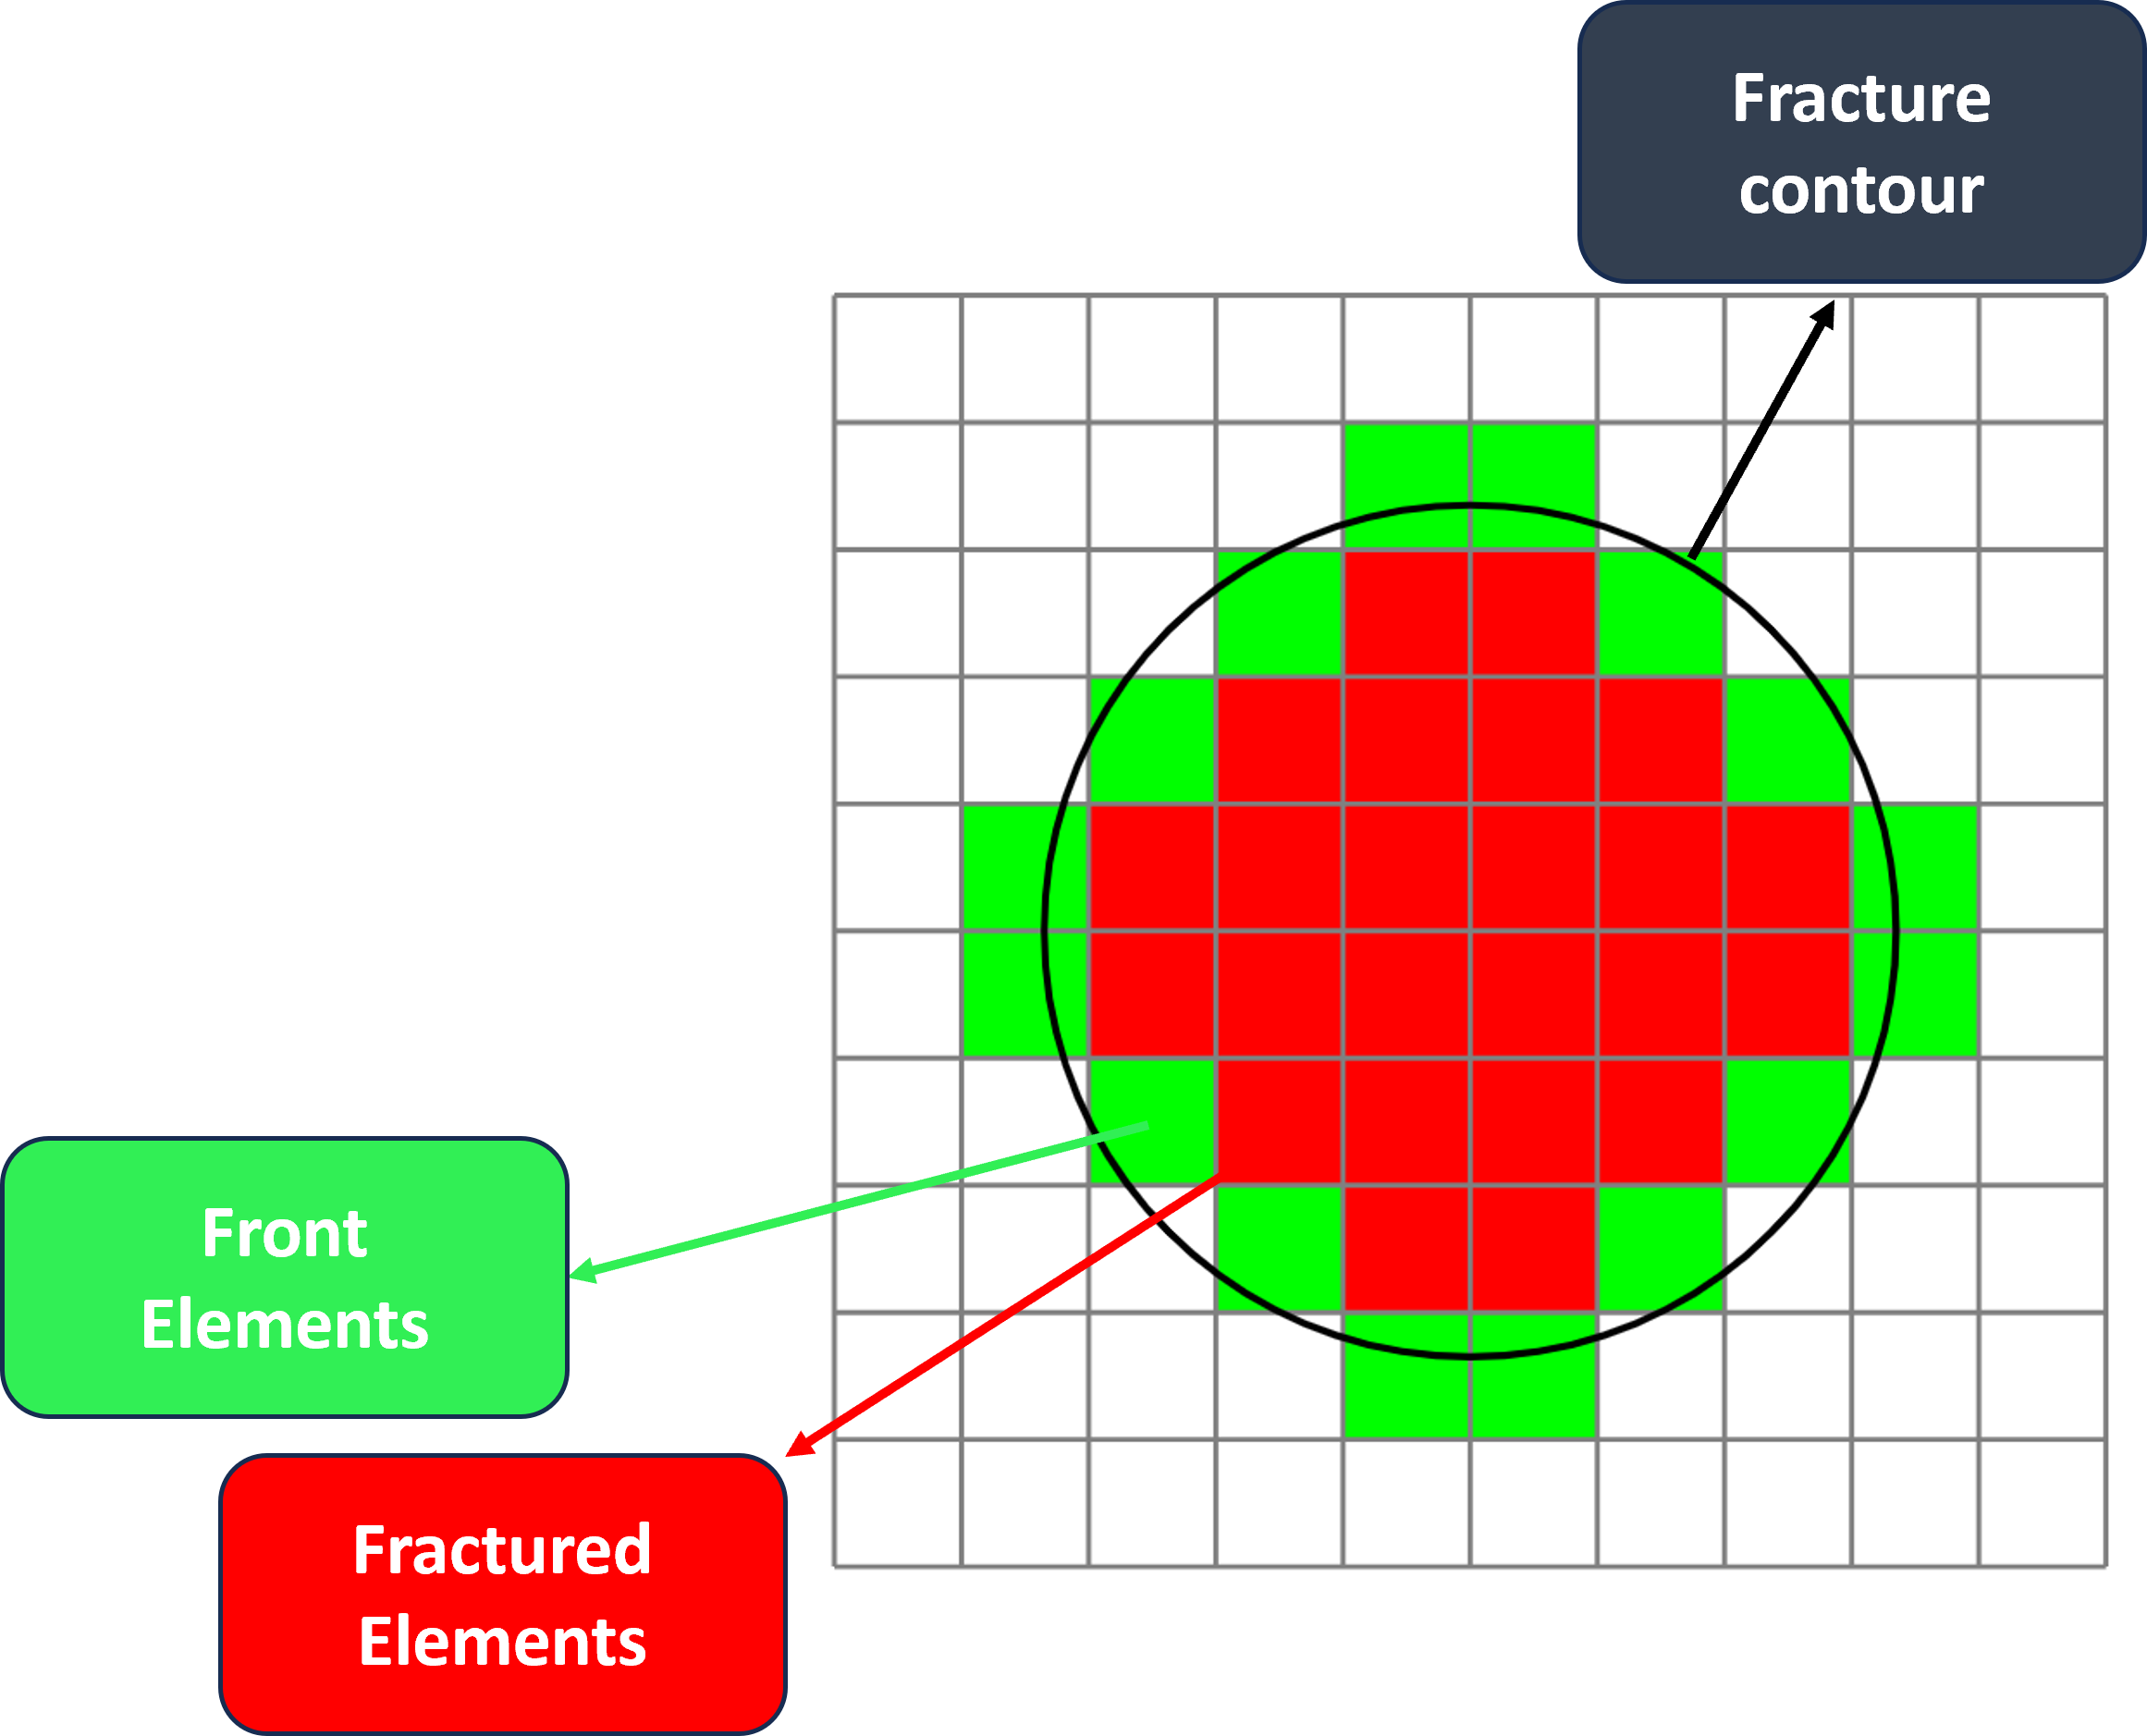
\includegraphics[width=\linewidth]{Chapter4/figures/penny_with_descriptions.png}
    \caption{Multi-resolution solution algorithm.}
    \label{fig:lorem4}
\end{figure}

\begin{figure}[h]
    \centering
    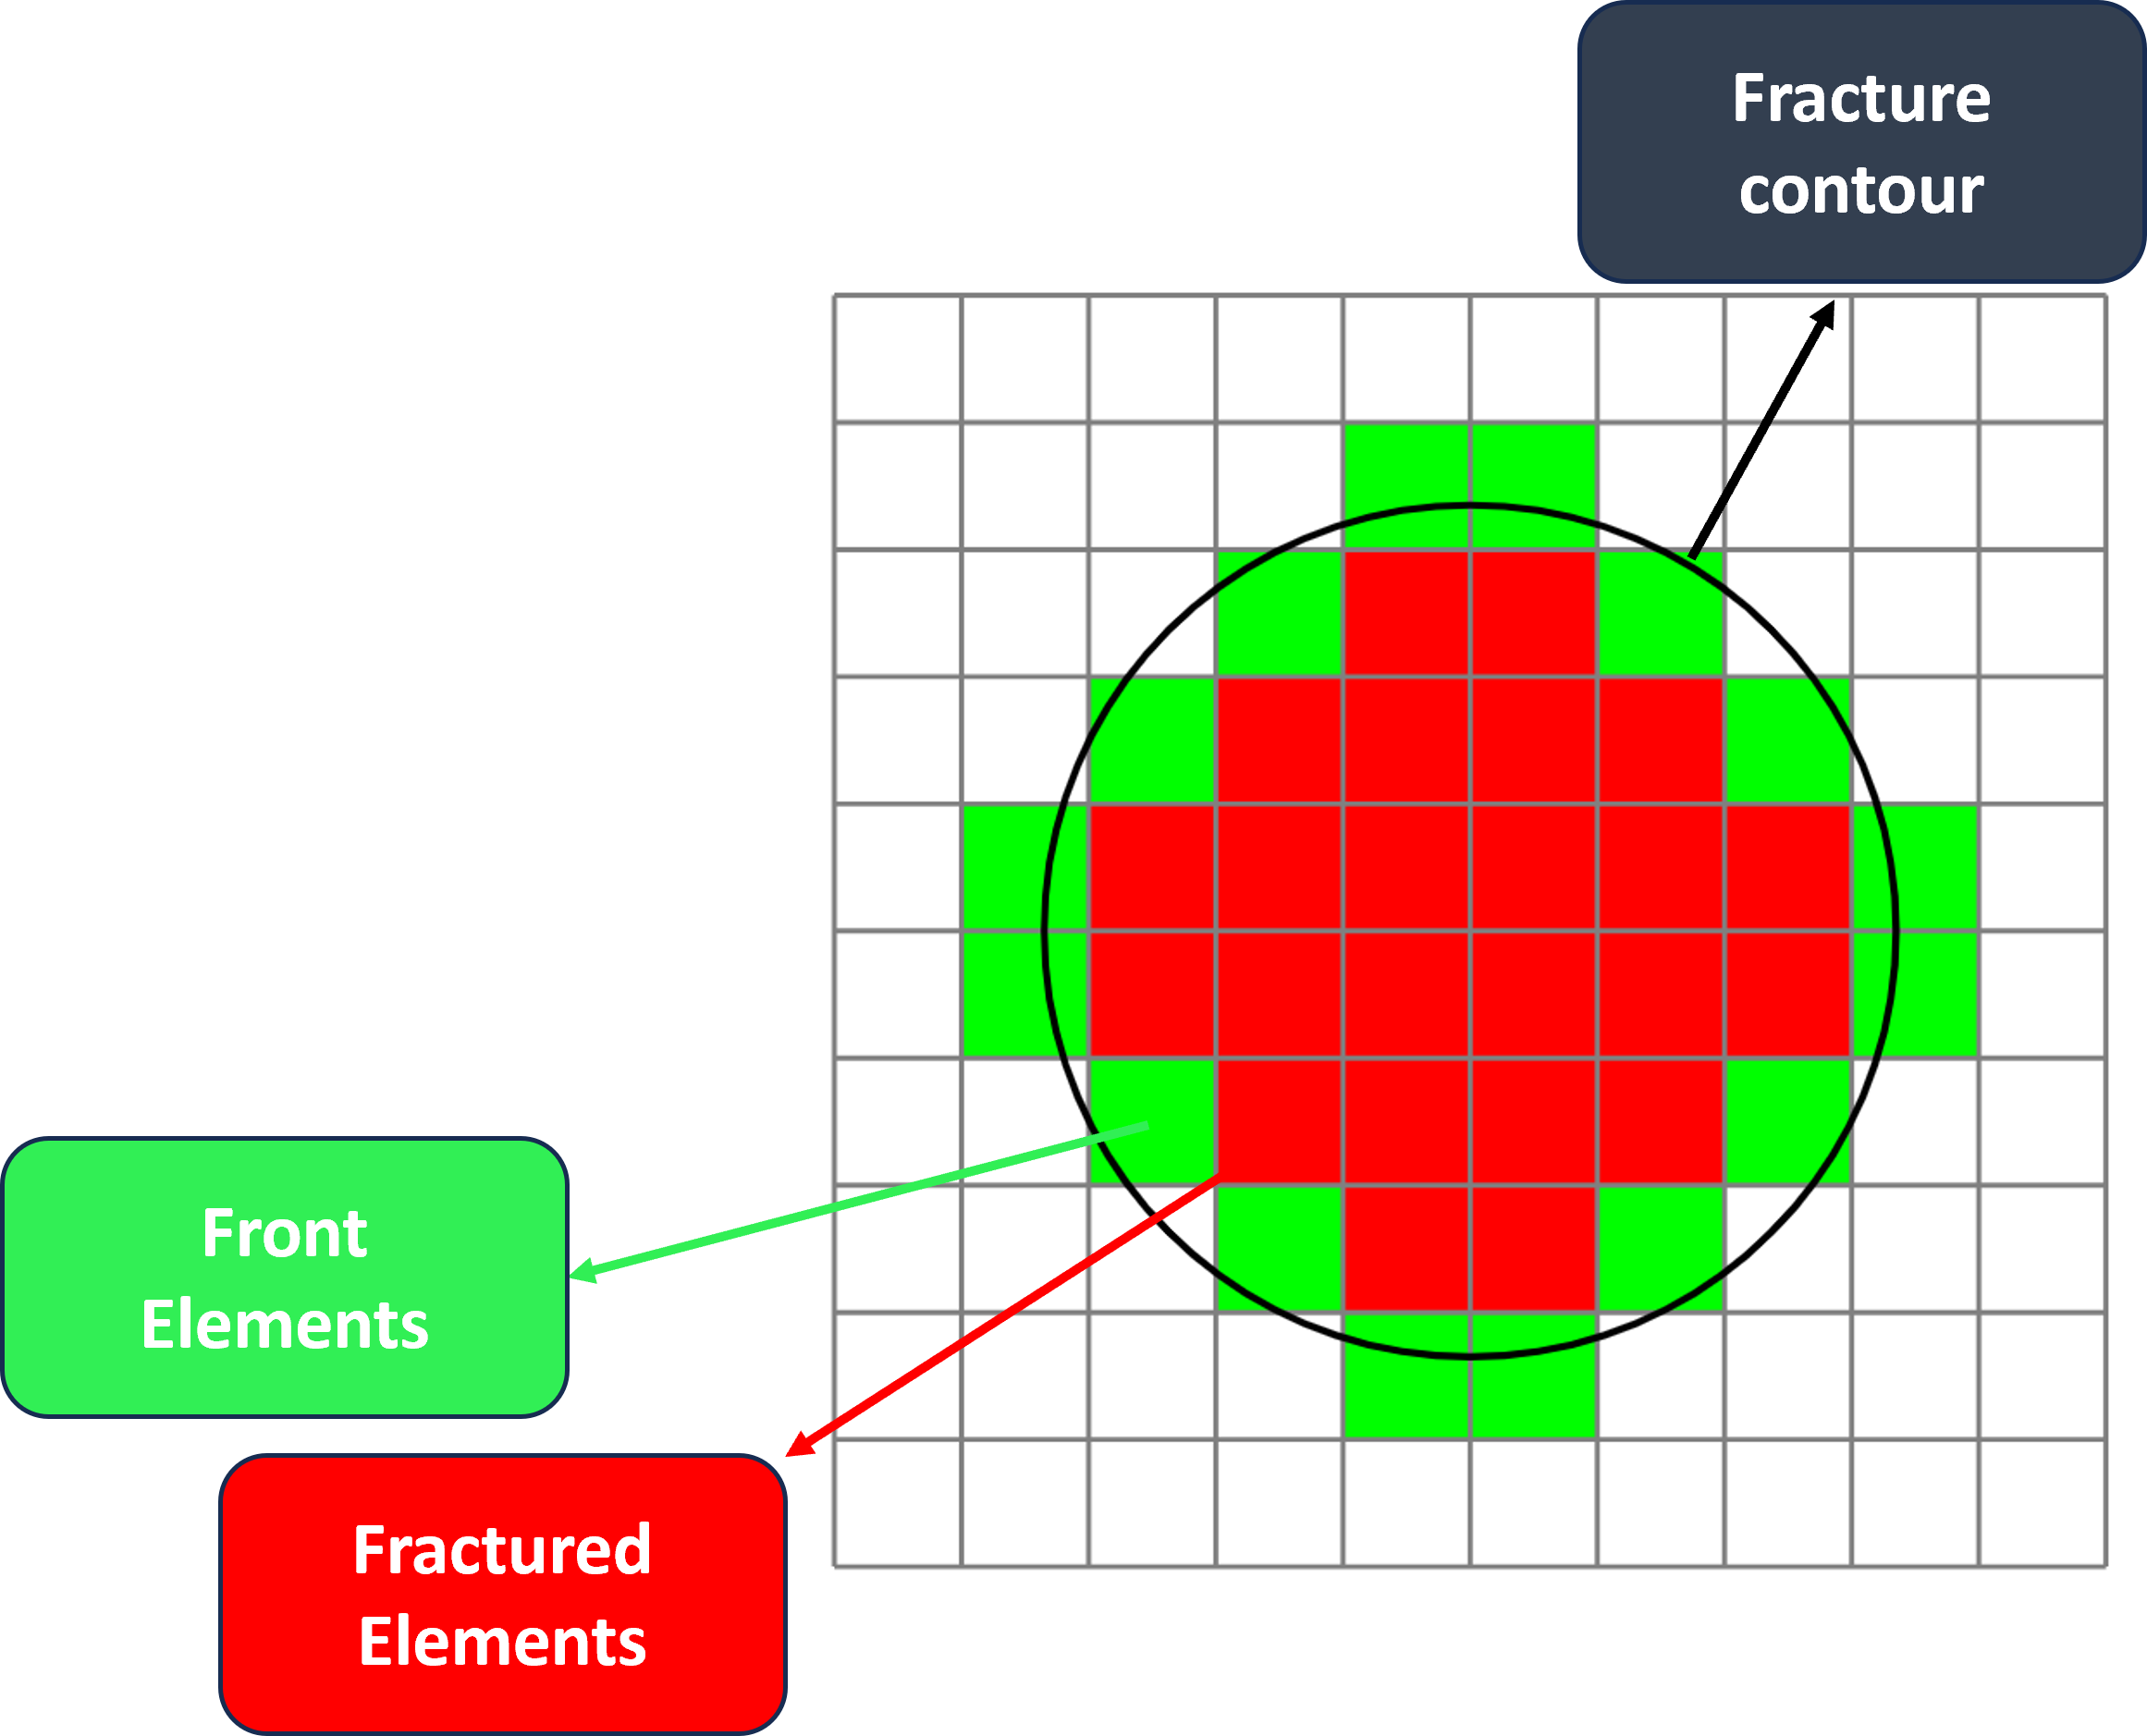
\includegraphics[width=\linewidth]{Chapter4/figures/penny_with_descriptions.png}
    \caption{Multi-resolution solution algorithm.}
    \label{fig:lorem4}
\end{figure}

\begin{figure}[h]
    \centering
    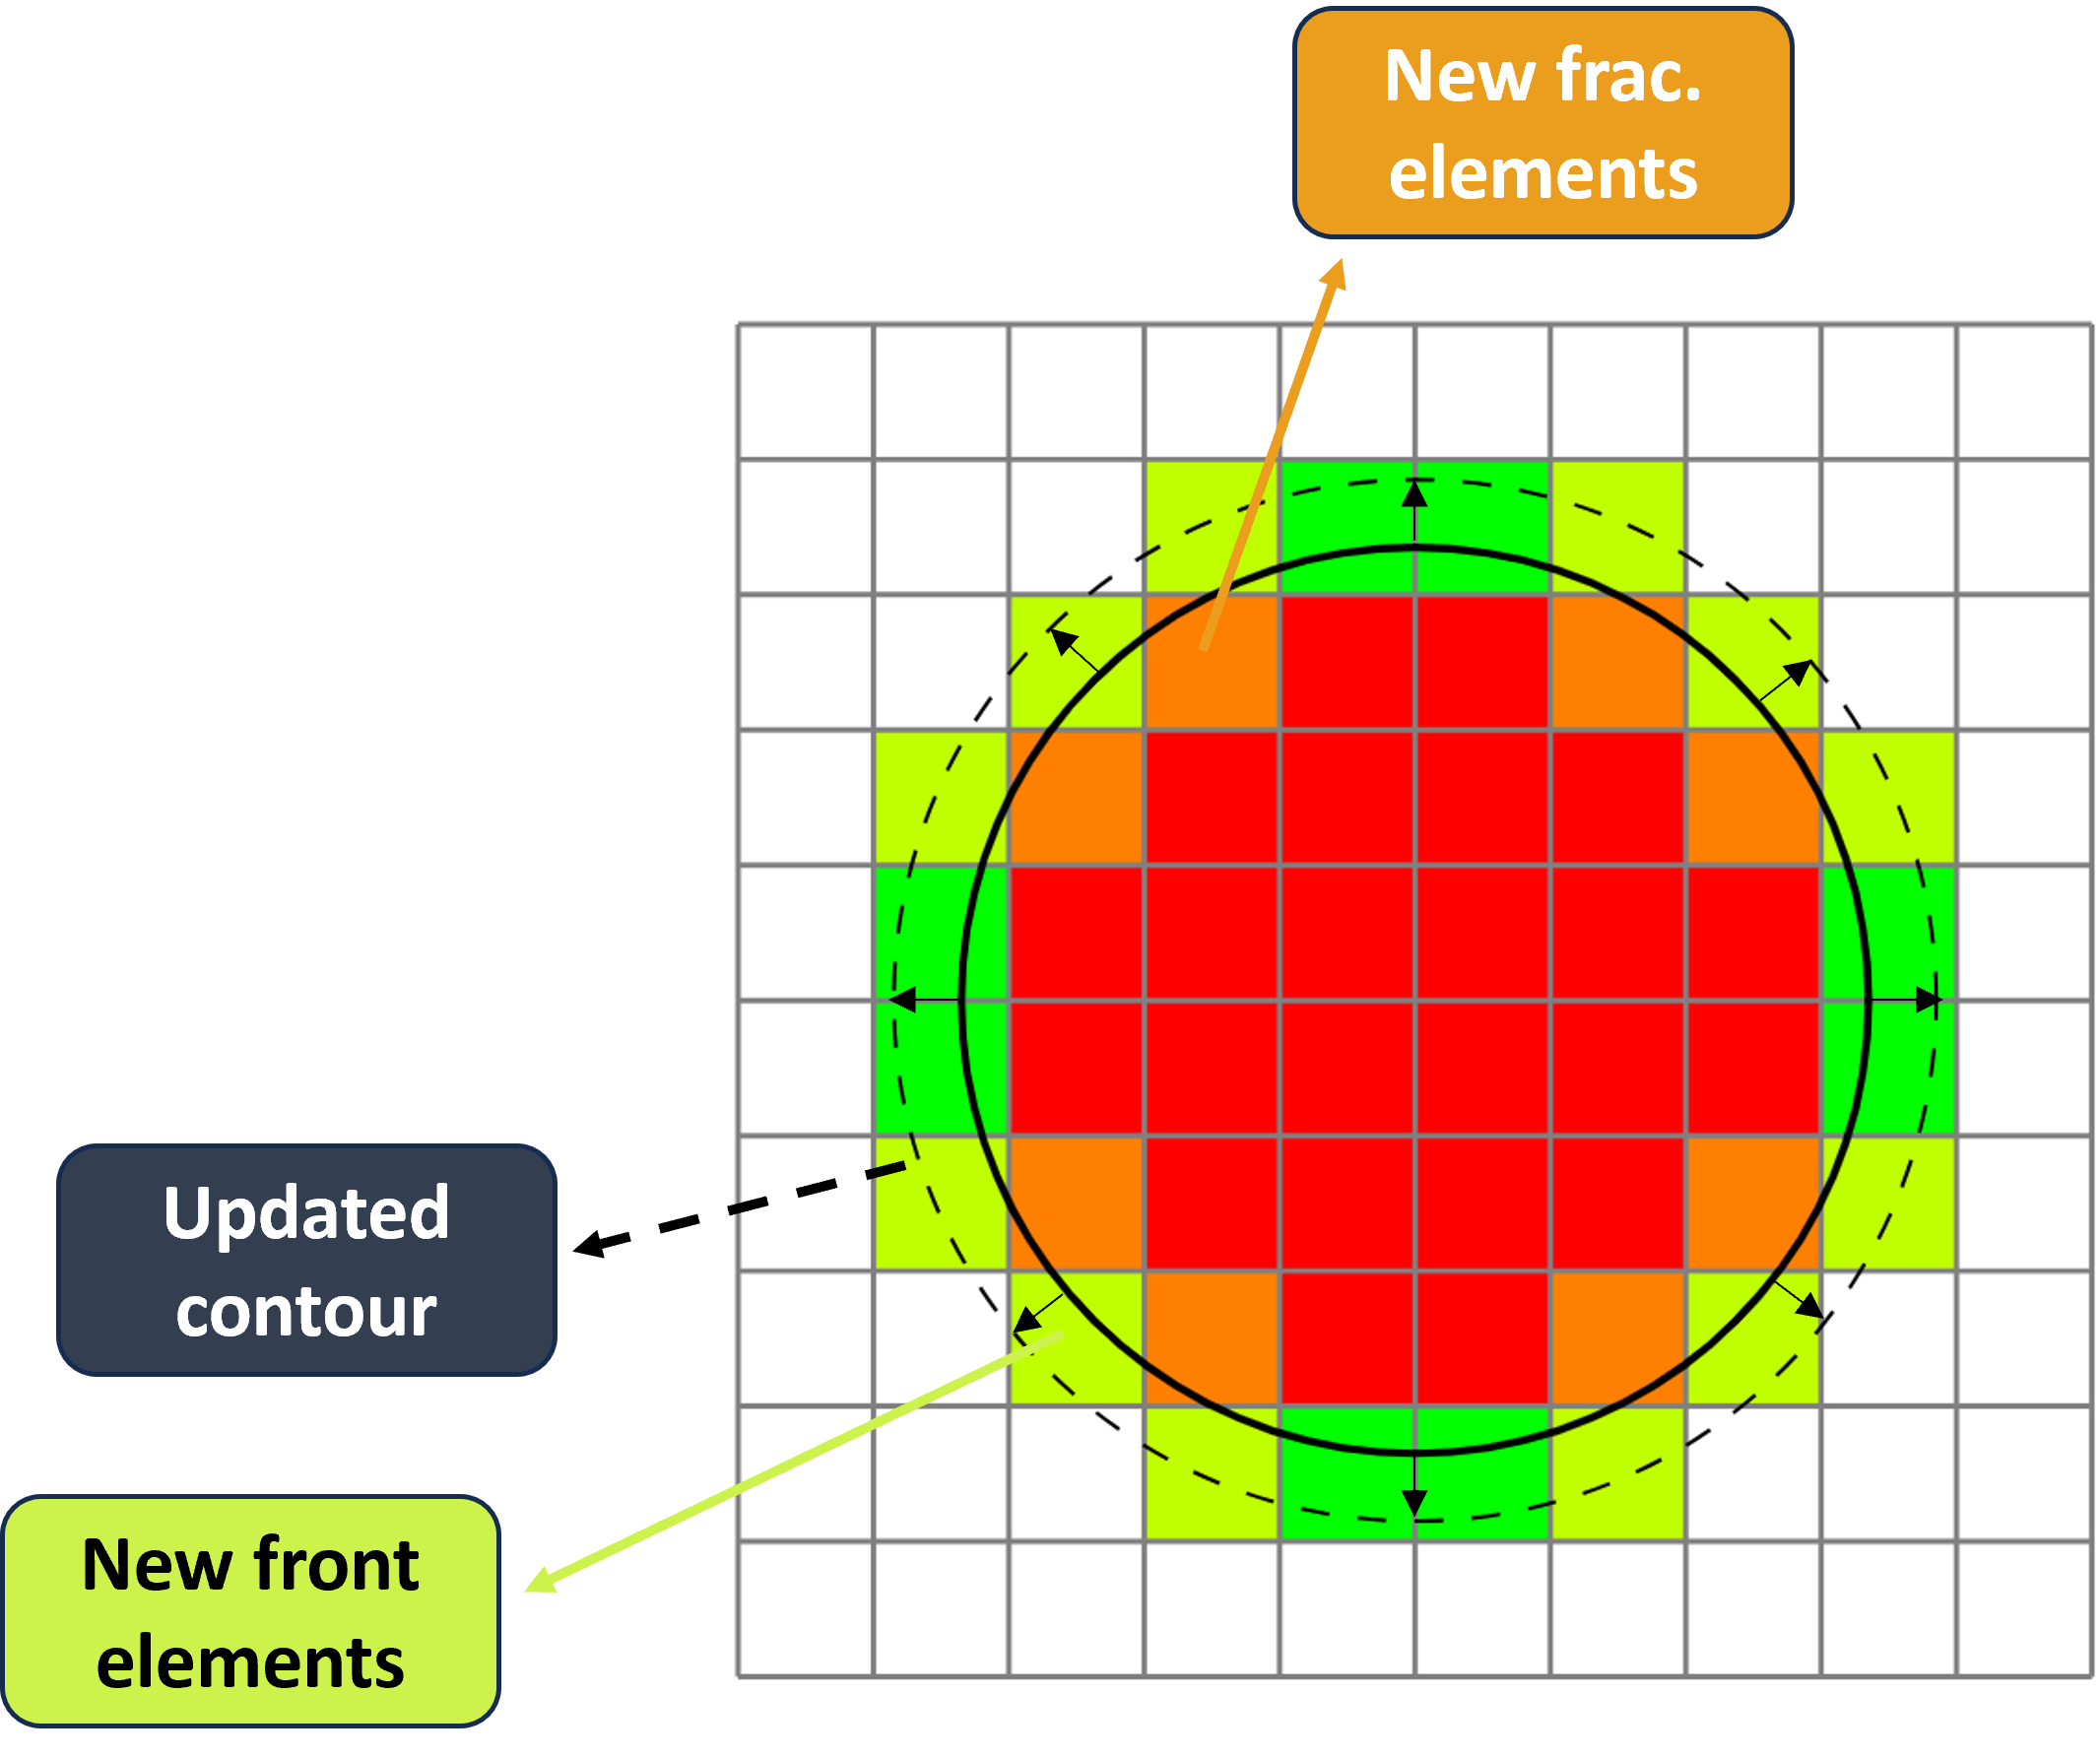
\includegraphics[width=\linewidth]{Chapter4/figures/larger_penny_with_descriptions.png}
    \caption{Multi-resolution solution algorithm.}
    \label{fig:lorem2}
\end{figure}

\begin{figure}[h]
    \centering
    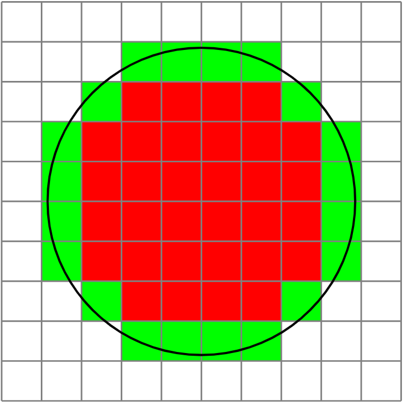
\includegraphics[width=0.5\linewidth]{Chapter4/figures/larger_penny.png}
    \caption{Multi-resolution solution algorithm.}
    \label{fig:lorem3}
\end{figure}

\begin{figure}[h]
    \centering
    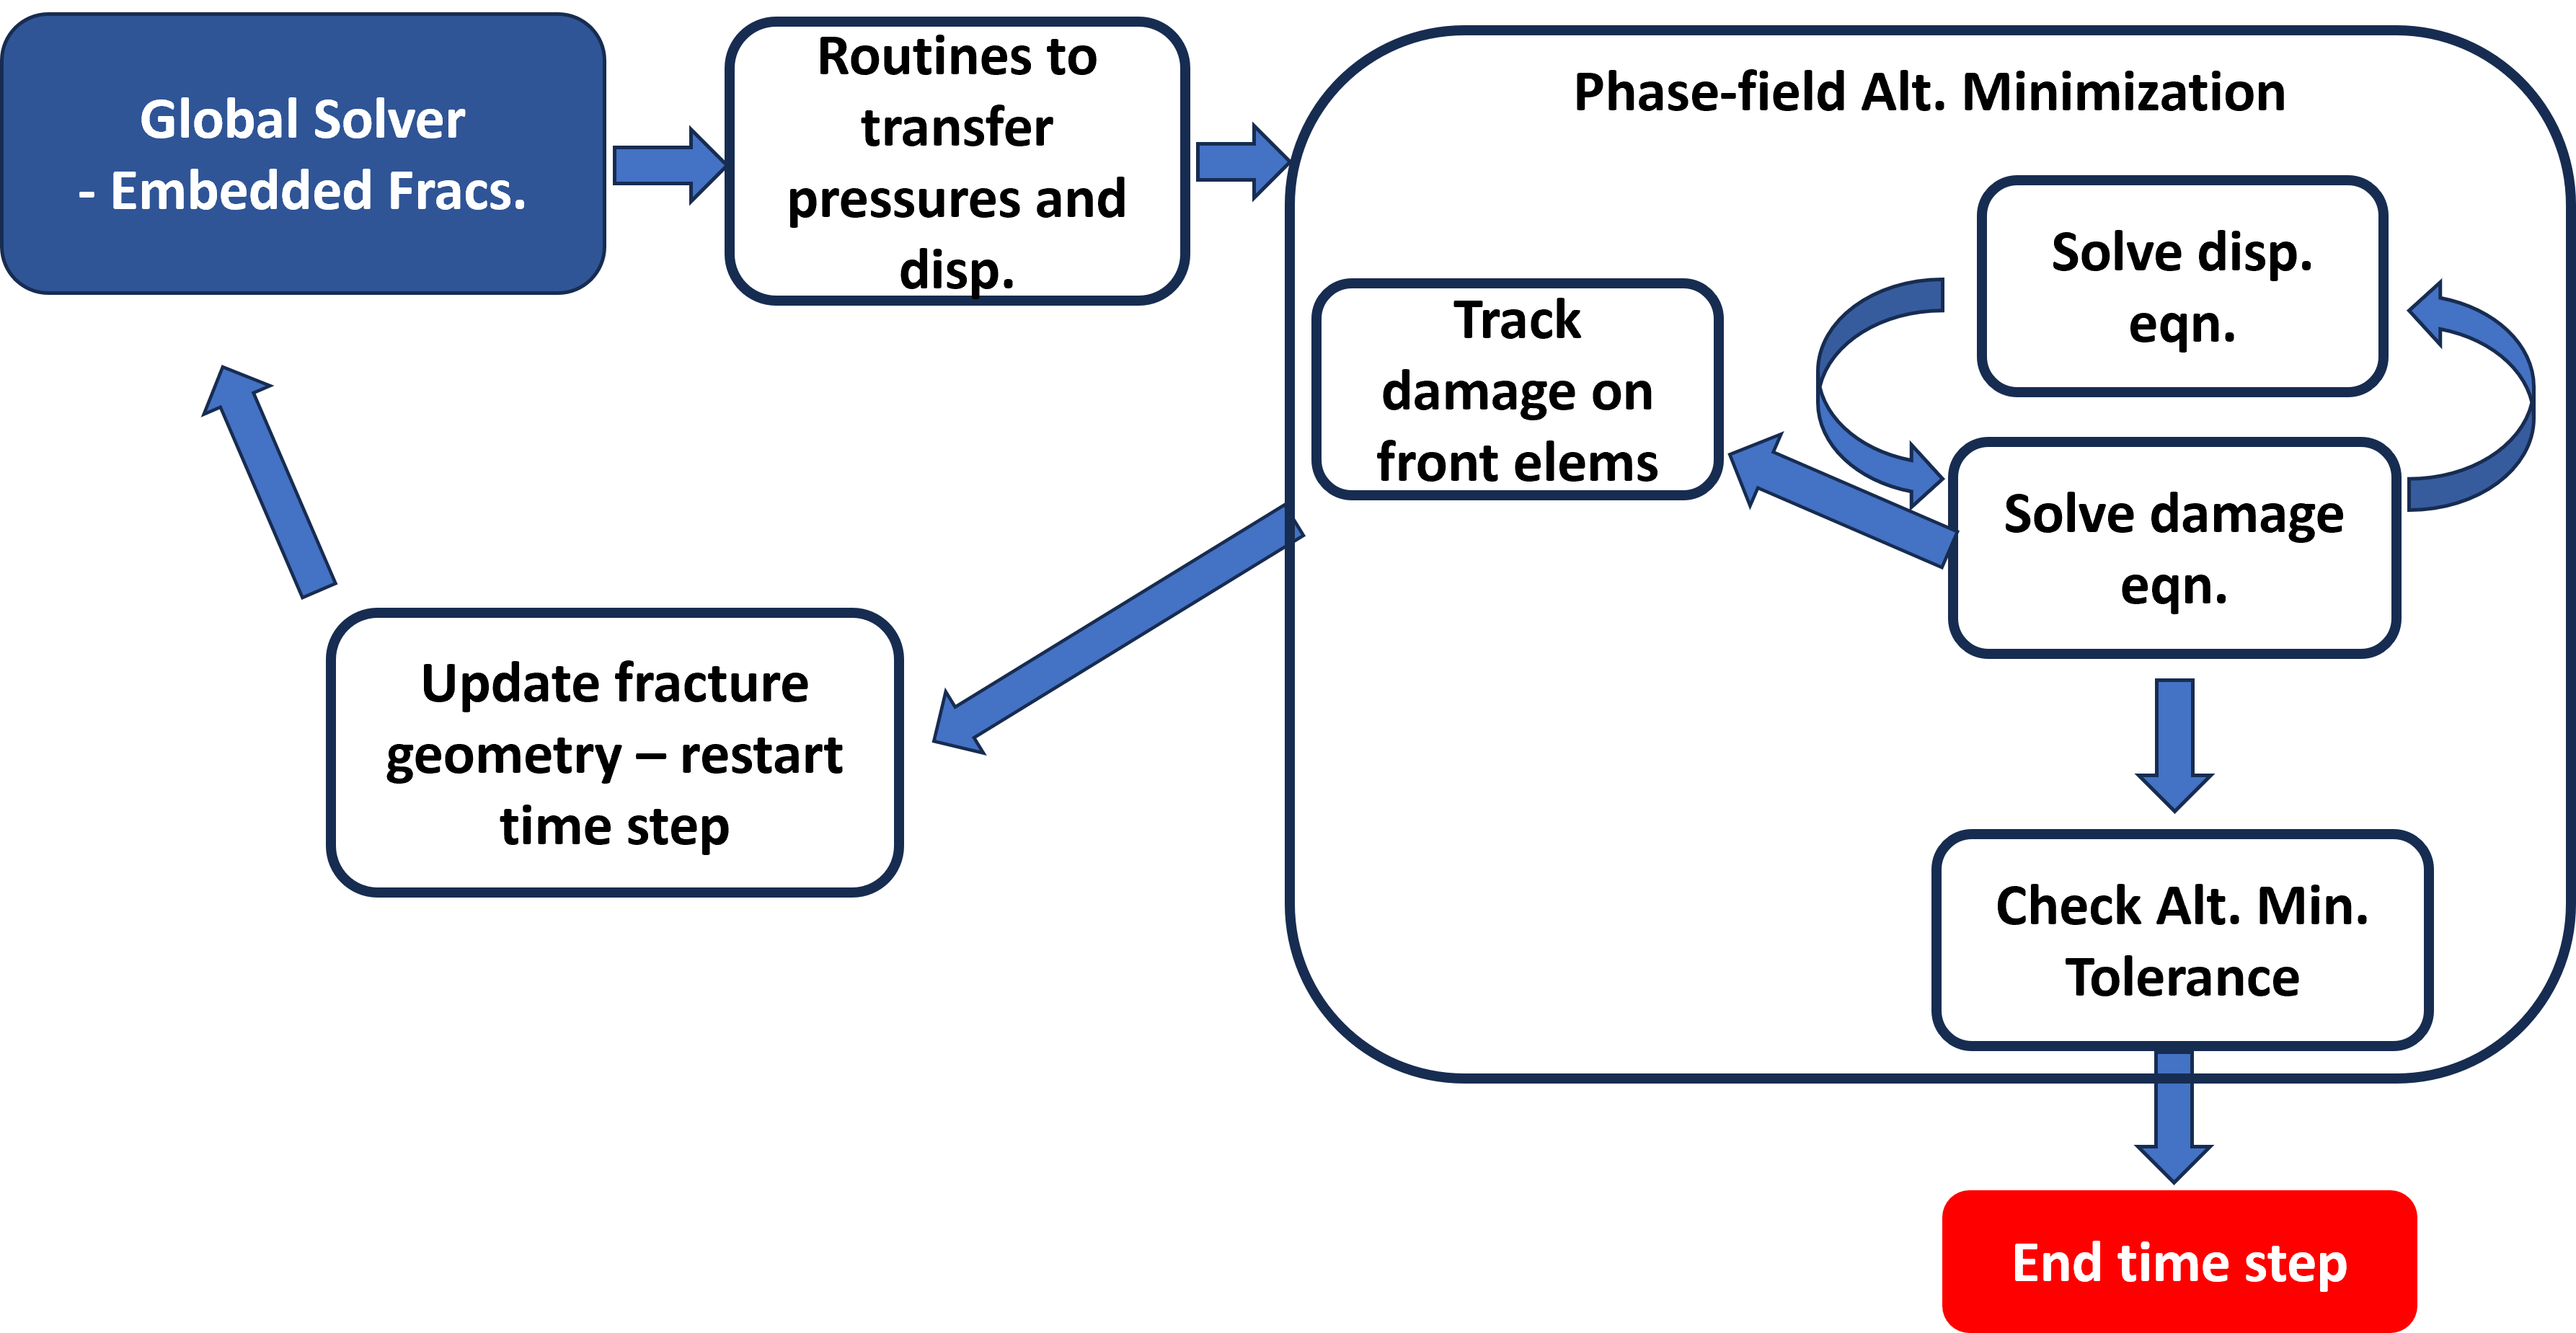
\includegraphics[width=\linewidth]{Chapter4/figures/planar3D_algorithm.png}
    \caption{Multi-resolution solution algorithm.}
    \label{fig:lorem5}
\end{figure}
